\scanpage{64}
% block: numerical characters item 3
\handwritten{3}) La donnée de l'application
\[
\handwritten{\sigma\unsure{\mathrel{\begin{tikzpicture}[x=1cm,y=1cm,baseline=-.05cm]\draw[thin] (0,-.13)--(0,.15);\draw[thin] (0,0)--(.52,0).. controls (.57,0) and (.58,.03)..(.59,.08);\end{tikzpicture}}|\mapsto}}(Z_{\handwritten{\sigma}},\handwritten{\xi_\sigma})\ ,\ \handwritten{\xi_\sigma\in}\operatorname{Br}(Z_{\handwritten{\sigma}})
\]
envisagée dans a).

% block: numerical characters item 4
4) La donnée de la fonction
\[
\operatorname{rang}\ :\ \handwritten{\mathcal{M}\longrightarrow}\underline{Z}
\]
lorsque $\handwritten{\mathcal{M}}$ est supposée\deleted{semi-}tannakienne.\deleted{\unsure{(i.e.}}

% block: effective part
On notera que la donnée de 1),2) équivaut à la donnée de l'anneau commutatif $K=K(\handwritten{\mathcal{M}})$, avec sa ``partie effective
\[
\begin{aligned}
K^{\mathrm{eff}}&=\text{sous-groupe de }K(\handwritten{\mathcal{M}})\text{ engendré par les}\\
&\qquad c\handwritten{\ell}(M),\ M\handwritten{\in}\operatorname{Ob}\quad,\\
&=\underline{N}^{(\handwritten{\Sigma})}
\end{aligned}
\]
(NB $\handwritten{\Sigma}$ se récupère à partir de \deleted{\unsure{ces}}\inserted{\handwritten{la}} donnée\inserted{\handwritten{$K^{\mathrm{eff}}\subset K$\begin{tikzpicture}[x=1cm,y=1cm,baseline=-.1cm]\draw[thin] (0,.12).. controls (.05,-.08) and (-.1,-.1)..(-.5,-.12)--(-1.6,-.12).. controls (-1.85,-.12) and (-1.95,-.28)..(-1.93,-.5);\end{tikzpicture}}} comme l'ensemble des éléme\unsure{nts} non nuls minimaux de $K^{\mathrm{eff}}$). La donnée de 3) permet alors de trouver, comme explicité dans a), la variance fonctorielle de l'anneau $K(\handwritten{\mathcal{M}}_{k'})$ par rapport à $k'$. Enfin la donnée de 4) permet en principe de retrouver les polynômes caractéristiques (en particulier, la trace et le déterminant) d'un endomorphisme d'un objet \deleted{de}(semi-simple ?) $M$ de $E$, en \unsure{\deleted{e}t|\deleted{o}t|\deleted{t}e}ermes de polynômes caractéristiques réduits (resp. trace réduite, norme réduite) dans les algèbres d'Azumaya\inserted{$\operatorname{End}(M_i)$,\begin{tikzpicture}[x=1cm,y=1cm,baseline=-.1cm]\draw[thin] (0,.12).. controls (.05,-.08) and (-.1,-.1)..(-.5,-.12)--(-1.6,-.12).. controls (-1.85,-.12) and (-1.95,-.28)..(-1.93,-.5);\end{tikzpicture}} correspondant aux composantes isotypiques $M_i$ de $M$. Pour $M$ isotypique de rang $n$, on aura en effet, si $K=\operatorname{End}(M)$ a comme centre $Z$ de rang $r$ sur $k$, donc $n=n'\unsure{\deleted{d}r|\deleted{r}d}$, et $K$ de rang $d^2$ sur $Z$, avec $d\handwritten{\mid}n'$ (NB $M$ de rang $n'$ sur $Z$):
\diagram{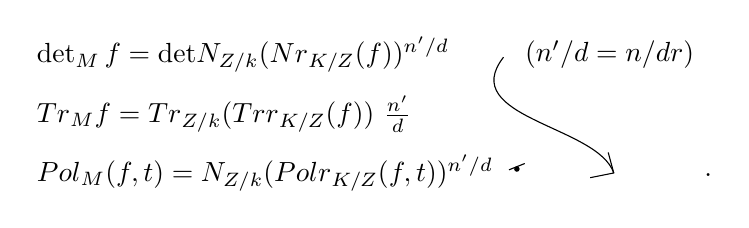
\begin{tikzpicture}[x=1cm,y=1cm]
\node[anchor=west] at (0,0) {$\det_M f=\deleted{\det}N_{Z/k}(\operatorname{Nr}_{K/Z}(f))^{n'/d}$};
\node[anchor=west] at (0,-.75) {$\operatorname{Tr}_M f=\operatorname{Tr}_{Z/k}(\operatorname{Trr}_{K/Z}(f))\ \frac{n'}{d}$};
\node[anchor=west] at (0,-1.5) {$\operatorname{Pol}_M(f,t)=N_{Z/k}(\operatorname{Polr}_{K/Z}(f,t))^{n'/d}$};
\node[anchor=west] at (6.2,0) {$\inserted{(n'/d=n/dr)}$};
\draw[thin] (6.05,-.03).. controls (5.45,-.8) and (7.25,-.9)..(7.45,-1.5);
\draw[thin] (7.15,-1.56)--(7.45,-1.5)--(7.38,-1.24);
\draw[thin] (6.12,-1.46)--(6.32,-1.38);\fill (6.22,-1.45) circle (.035);
\node at (8.65,-1.52) {$.$};
\end{tikzpicture}}
\margin{\handwritten{\unsure{Signaler} que la connaissance des car. num. de $\mathcal{M}$ implique celle des car. numériques de $\mathcal{M}_{k'}$ pour \unsure{toute} extension $k'$ de $k$, (``fonctorielle en $k'$'')}}

% block: warning about reconstruction
On fera attention que la connaissance des caractères numériques de la catégorie tannakienne $\handwritten{\mathcal{M}}$ ne permet pas en général de réconstituer celle-ci à équivalence près, même si $k$ est un corps alg. clos de car. 0 (de sorte que la donnée de 3) devient vide) et $\handwritten{\mathcal{M}}$ semi-simple
% archive sheet number: 63
